\documentclass[12pt]{article}

\usepackage{fullpage}
\usepackage{multicol,multirow}
\usepackage{tabularx}
\usepackage{ulem}
\usepackage{graphicx}%Вставка картинок правильная
\usepackage{float}%"Плавающие" картинки
\usepackage{wrapfig}%Обтекание фигур (таблиц, картинок и прочего)
\usepackage[utf8]{inputenc}
\usepackage[russian]{babel}

% Оригиналный шаблон: http://k806.ru/dalabs/da-report-template-2012.tex

\begin{document}

\section*{Курсовой проект по курсу дискрeтного анализа: Текстовый поиск}

Выполнил студент группы 08-307 МАИ \textit{Дегтярев Денис Андреевич}.

\subsection*{Условие}

Ваша программа должна читать входные данные из стандартного потока ввода и выводить ответ на стандартный поток вывода.
Реализуйте инвертированный индекс, затем проведите поиск текстов содержащих заданные наборы слов.

\subsection*{Формат ввода}

В первой строке входного файла вам дано число n — количество текстов. В следующих 
n строках даны тексты, по одному тексту в строке, представленные наборами слов разделёнными пробелами. Далее задано 
m
 — количество запросов в файле. В следующих 
m
 строках вам даны запросы по одному в строке представленные наборами слов разделённых пробелами.  

 \subsection*{Формат вывода}

В ответ на каждый запрос выведите список подходящих документов в виде: c i — количество подходящих под запрос документов и далее номера текстов в которых встречались все слова из i-го запроса. Нумерация документов начинается с 0.  

\subsection*{Метод решения}

Для решения задачи текстового поиска для начала читаем каждый текст и в хэш таблицу \texttt{unordered\_map} к каждому слову, встреченному в тексте, заносим в очередь индекс данного текста. 
В итоге мы получаем \texttt{unordered\_map}, где ключами являются слова, а их значениями - queue, состоящие из индексов, соответствующих текстов.  
Далее, на этапе запросов, программа последовательно считывает слова из строки и получает пересечение полученных queue для каждого слова. В итоге, на выходе выводится размер queue, 
в котором хранятся индексы текстов, в которых встречалоись все заданные слова строки, и соответствующие индексы.

\subsection*{Описание программы}

Функция intersection выводит пересечение очередей (причем, тк индексы - алгебраическая прогрессия с шагом 1, можно сказать, что очередь отсортирована).  
В main происходят все считывания и основные вычисления для решения задачи.

\subsection*{Дневник отладки}  

Несколько попыток было потрачено на WA. Как оказалось, я перепутал метод front и back для очереди, в связи с чем queue для каждого из слов имел некоторые не уникальные индексы, что привело к неверному ответу. 
После исправления ошибки тесты были пройдены. 
Затем, я решил проверить, сколько текстов всего могло бы быть в запросах. Как оказалось, их меньше 32767, за счет чего я уменьшил объем занимаемой памяти и скорость работы программы.

\subsection*{Тест производительности}

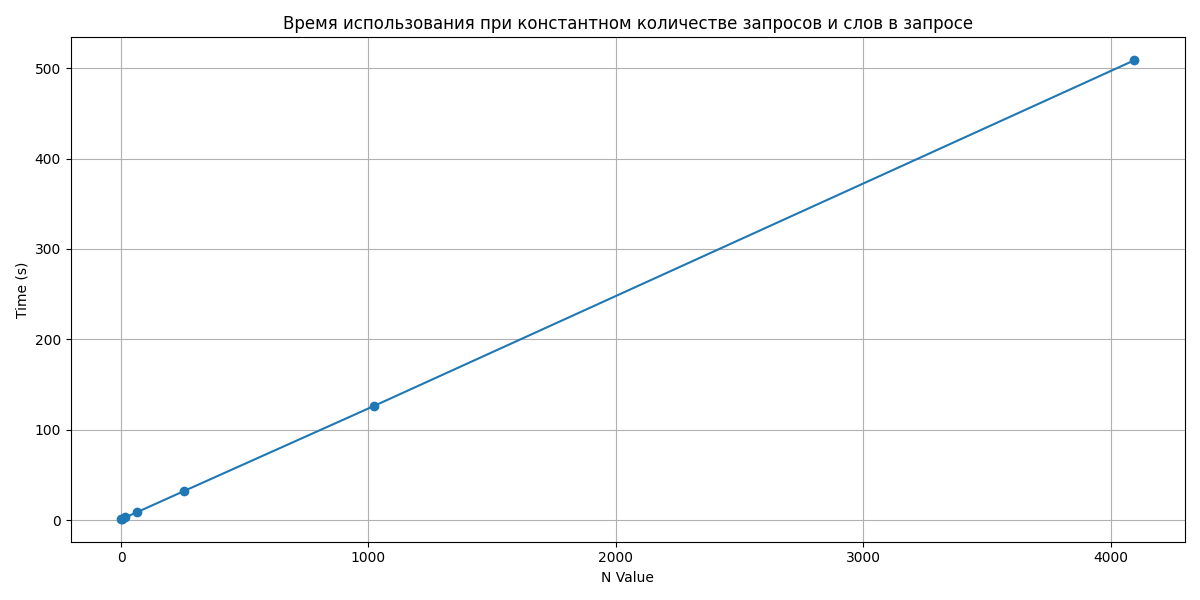
\includegraphics[width=7in]{Figure_1.png}

\subsection*{Особенности программы}

Все операции вставки выполняются в среднем за \( O(1) \), если не брать в оборот ситуации коллизий (их вероятность мала).
Все операции поиска выполняются за \( O\left(\sum_{i=1}^{k} \text{queue}_i.\text{size}()\right) \), где k - количество слов в строке.  
То есть, при одном слове в строке поиска, поиск будет выполняться за \( O(1) \).

\subsection*{Выводы}

В процессе реализации инвертированного индекса и алгоритма поиска по текстам для написания курсового проекта по предмету «Дискретный анализ» я достиг нескольких важных целей и узнал много нового:

\begin{enumerate}
    \item \textbf{Понимание инвертированных индексов}: Я получил глубокое понимание того, как работают инвертированные индексы, которые являются основой многих систем полнотекстового поиска. Это знание может быть применено в разработке поисковых систем и в обработке больших объёмов текстовых данных.
    \item \textbf{Работа с хэш-таблицами}: Я использовал \texttt{unordered\_map} для создания индекса, что помогло мне практически применить знания о хэш-таблицах, включая их эффективность и способы применения в реальных задачах.
    \item \textbf{Алгоритмическое мышление}: Решение задачи требовало алгоритмического подхода, в частности, для определения пересечения наборов текстов. Это укрепило мои навыки в области алгоритмов и структур данных.
    \item \textbf{Работа со строками и текстовыми данными}: Я практиковался в обработке и анализе строк, что полезно во многих областях программирования, от разработки программного обеспечения до анализа данных.
    \item \textbf{Проблемы масштабируемости и оптимизации}: Я столкнулся с вопросами масштабируемости и оптимизации при обработке большого количества текстов и запросов, что представляет собой важный аспект в разработке производительных приложений.
    \item \textbf{Умение решать практические задачи}: Я успешно применил теоретические знания для решения практической задачи, что является важным навыком в любой инженерной дисциплине.
\end{enumerate}

Таким образом, выполнение этой работы не только помогло мне развить технические навыки в области компьютерных наук, но и дало ценный опыт в решении реальных задач, который может быть применен в будущих проектах.

\end{document}
